%
% $RCSfile: idiomatic.tex,v $
%
% Copyright (c) 2004. Christian Heller. All rights reserved.
%
% No copying, altering, distribution or any other actions concerning this
% document, except after explicit permission by the author!
% At some later point in time, this document is planned to be put under
% the GNU FDL license. For now, _everything_ is _restricted_ by the author.
%
% http://www.cybop.net
% - Cybernetics Oriented Programming -
%
% http://www.resmedicinae.org
% - Information in Medicine -
%
% @author Christian Heller <christian.heller@tuxtax.de>
%

\subsubsection{Idiomatic}
\label{idiomatic_heading}

An \emph{Idiom} is a pattern on a low abstraction level. It describes how certain
aspects of components or the relations between them can be implemented using the
means of a specific programming language. Idioms can such be used to describe
the actual realization of design patterns. Besides the \emph{Counted-Pointer}
pattern, Buschmann \cite[p. 377]{buschmann} also categorizes \emph{Singleton},
\emph{Template Method}, \emph{Factory Method} and \emph{Envelope-Letter}
\cite{coplien} as \emph{Idiom}.

%
% $RCSfile: template_method.tex,v $
%
% Copyright (C) 2002-2008. Christian Heller.
%
% Permission is granted to copy, distribute and/or modify this document
% under the terms of the GNU Free Documentation License, Version 1.1 or
% any later version published by the Free Software Foundation; with no
% Invariant Sections, with no Front-Cover Texts and with no Back-Cover
% Texts. A copy of the license is included in the section entitled
% "GNU Free Documentation License".
%
% http://www.cybop.net
% - Cybernetics Oriented Programming -
%
% http://www.resmedicinae.org
% - Information in Medicine -
%
% Version: $Revision: 1.1 $ $Date: 2008-08-19 20:41:09 $ $Author: christian $
% Authors: Christian Heller <christian.heller@tuxtax.de>
%

\subsubsection{Template Method}
\label{template_method_heading}
\index{Template Method Pattern}
\index{Hook Method Pattern}

The \emph{Template Method} pattern \cite{gamma1995}, also called
\emph{Hook Method}, is an abstract definition of the \emph{Skeleton} of an
algorithm. The implementation of one or more steps of that algorithm is
delegated to a sub class (figure \ref{templatemethod_figure}).

\begin{figure}[ht]
    \begin{center}
        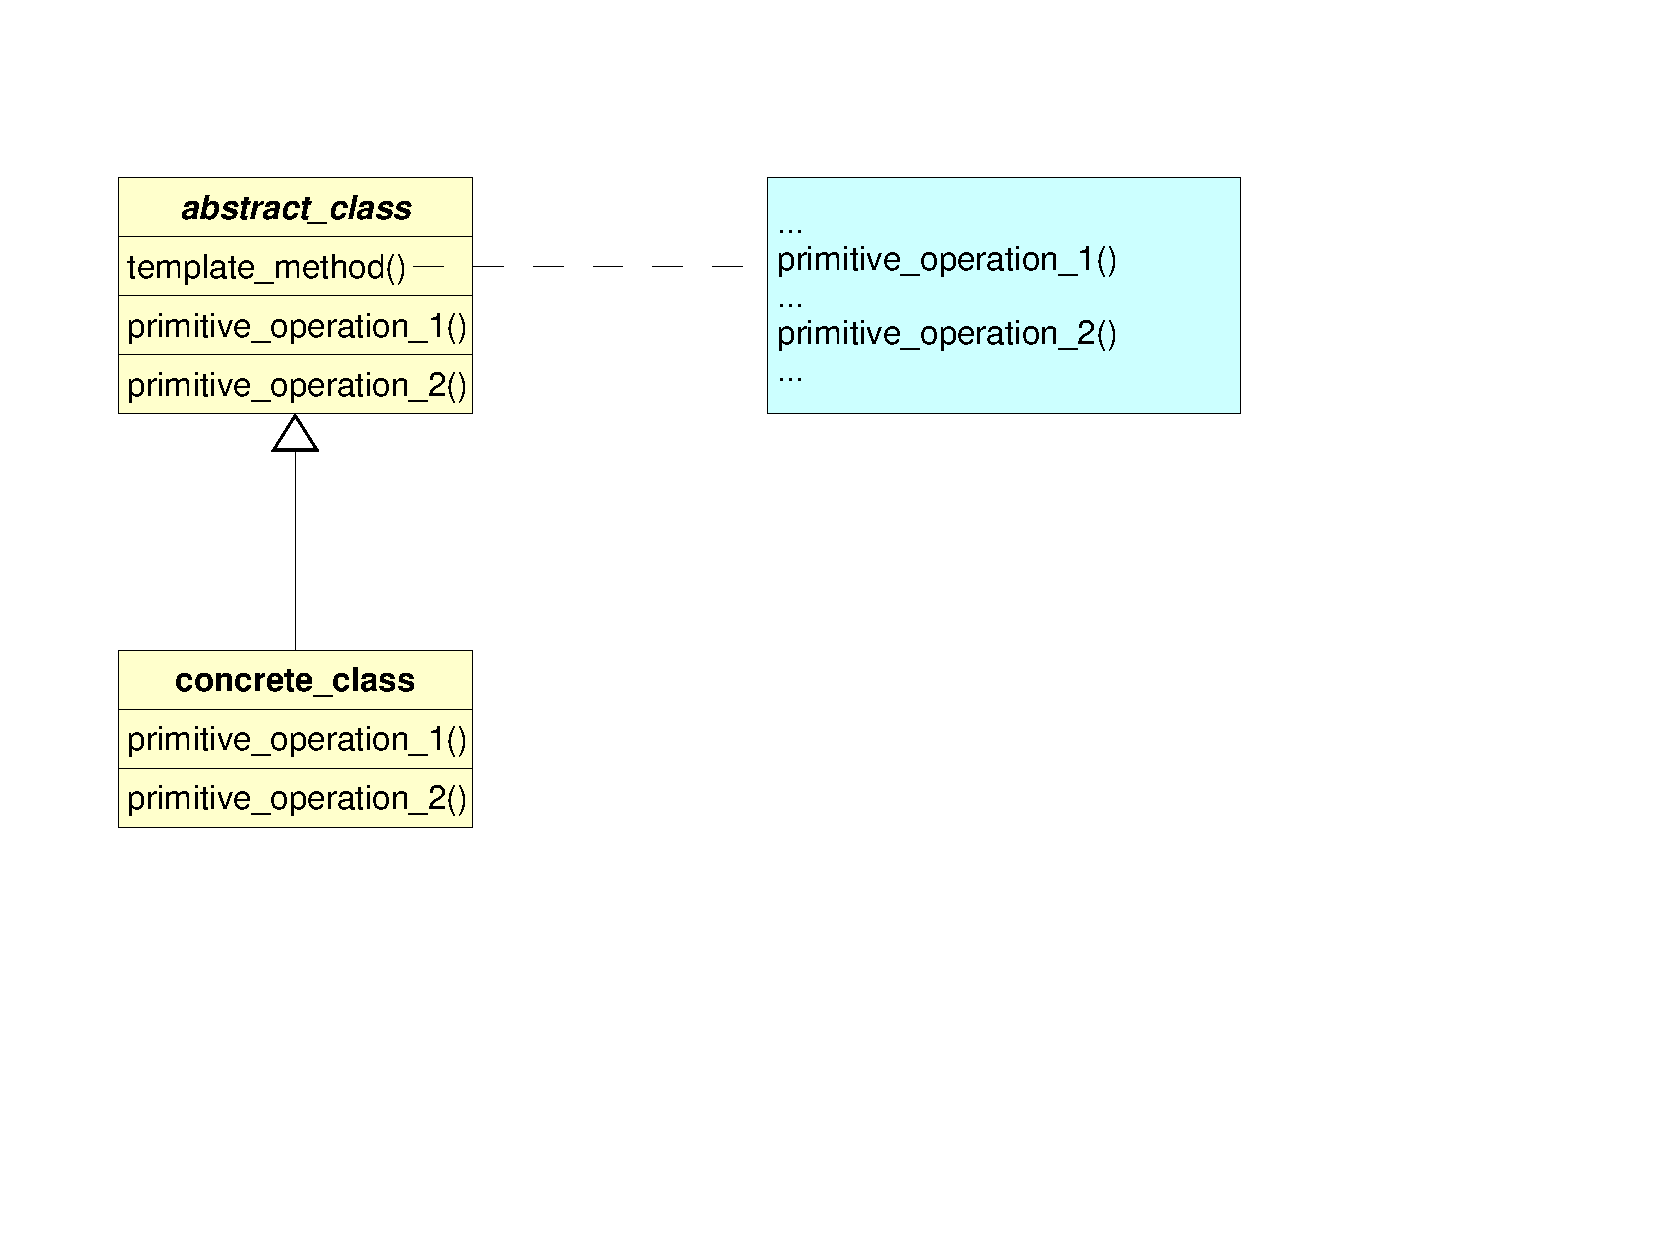
\includegraphics[scale=0.3,angle=-90]{graphic/templatemethod.pdf}
        \caption{Template Method Pattern}
        \label{templatemethod_figure}
    \end{center}
\end{figure}

The idea of algorithm (method) templates was taken over in the design of the
new language described in chapter \ref{cybernetics_oriented_language_heading}.
The single template parts, however, are not inherited but implemented in
\emph{part} templates referenced by their corresponding \emph{whole} template,
which is actually more similar to the previously described \emph{Whole-Part}
pattern (section \ref{design_heading}).

%
% $RCSfile: counted_pointer.tex,v $
%
% Copyright (c) 2004. Christian Heller. All rights reserved.
%
% No copying, altering, distribution or any other actions concerning this
% document, except after explicit permission by the author!
% At some later point in time, this document is planned to be put under
% the GNU FDL license. For now, _everything_ is _restricted_ by the author.
%
% http://www.cybop.net
% - Cybernetics Oriented Programming -
%
% http://www.resmedicinae.org
% - Information in Medicine -
%
% @author Christian Heller <christian.heller@tuxtax.de>
%

\paragraph{Counted Pointer}
\label{counted_pointer_heading}

The \emph{Counted Pointer} pattern \cite{buschmann} supports memory management
in the \emph{C++} programming language, by counting references to dynamically
created objects (figure \ref{pointer_figure}). That way, it can avoid the
destruction of an object through one client, while still being referenced by
other clients. Also, it helps avoiding memory leaks by cleaning up forgotten
objects.

\begin{figure}[ht]
    \begin{center}
        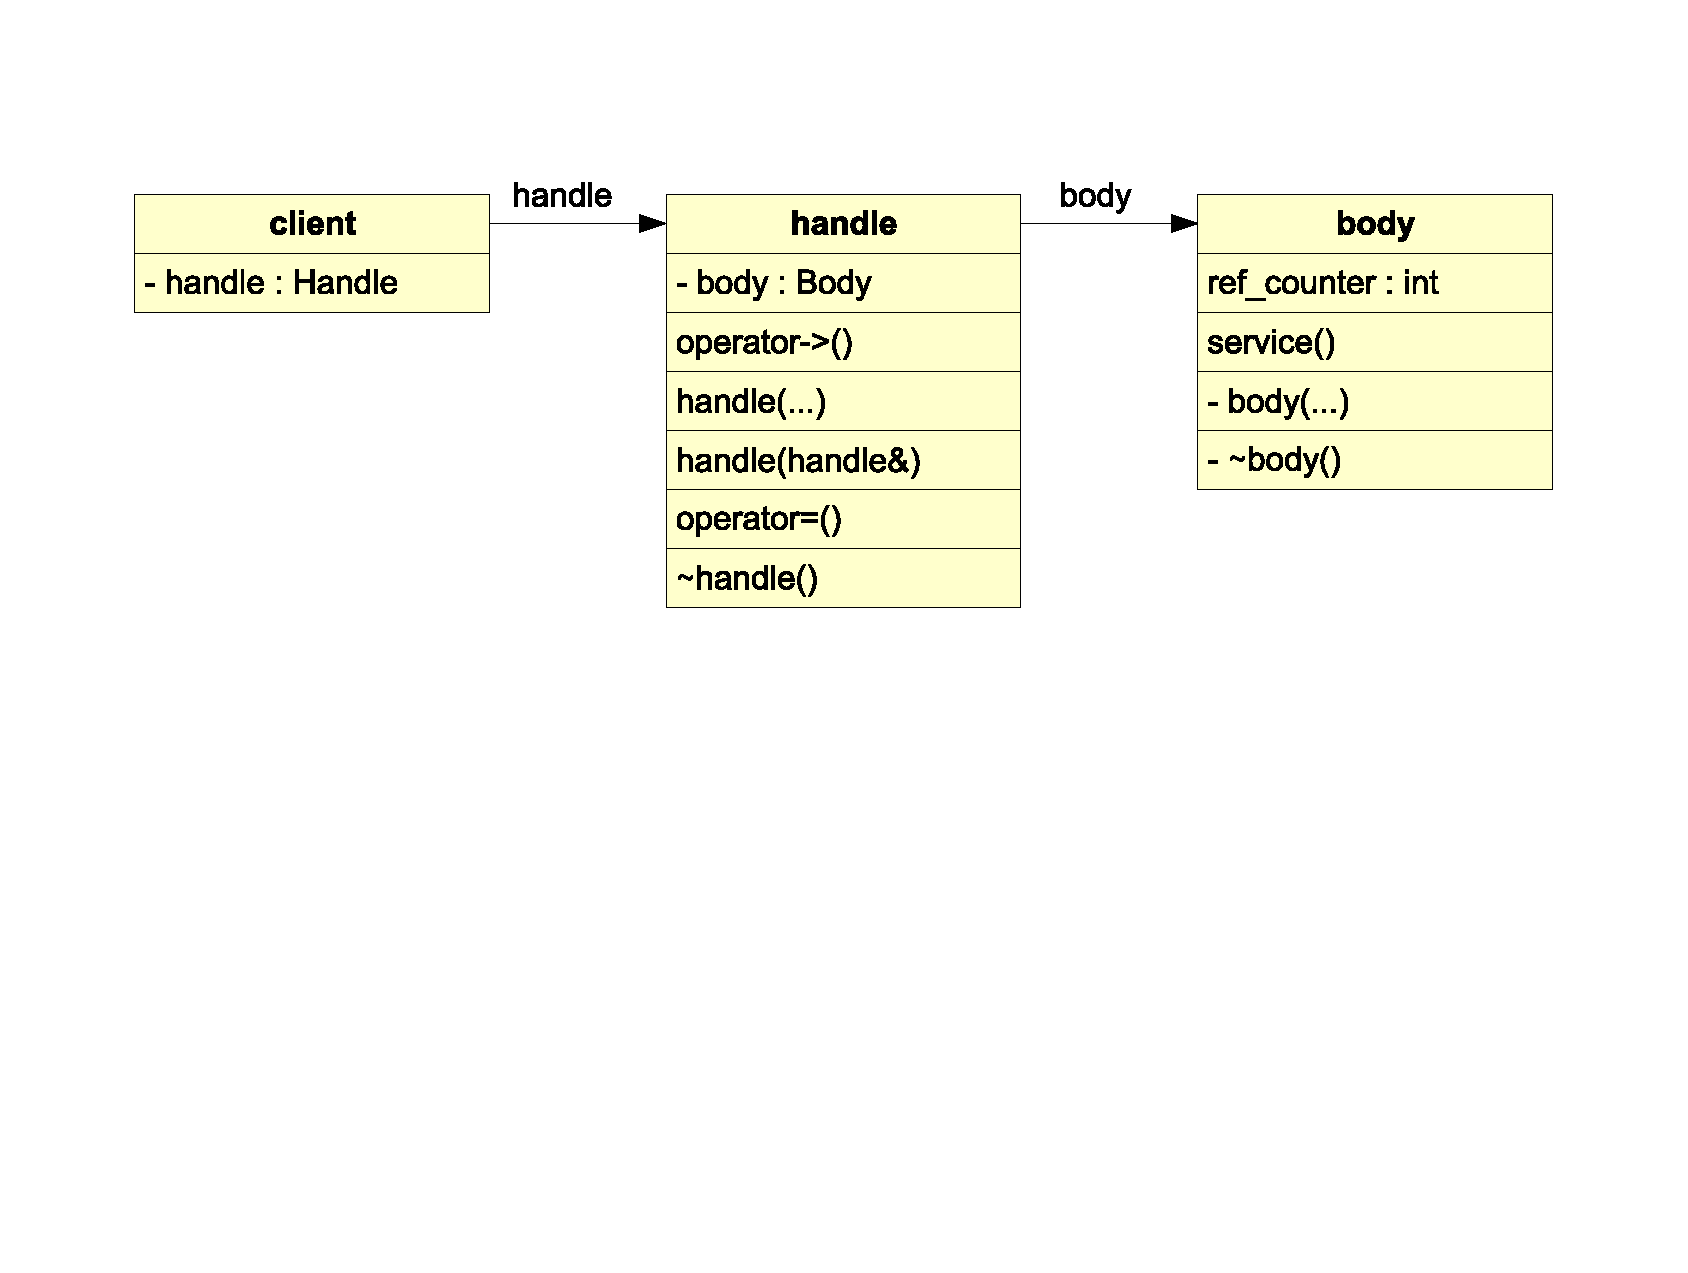
\includegraphics[scale=0.3]{vector/pointer.eps}
        \caption{Counted Pointer Pattern}
        \label{pointer_figure}
    \end{center}
\end{figure}

%
% $RCSfile: singleton.tex,v $
%
% Copyright (C) 2002-2008. Christian Heller.
%
% Permission is granted to copy, distribute and/or modify this document
% under the terms of the GNU Free Documentation License, Version 1.1 or
% any later version published by the Free Software Foundation; with no
% Invariant Sections, with no Front-Cover Texts and with no Back-Cover
% Texts. A copy of the license is included in the section entitled
% "GNU Free Documentation License".
%
% http://www.cybop.net
% - Cybernetics Oriented Programming -
%
% http://www.resmedicinae.org
% - Information in Medicine -
%
% Version: $Revision: 1.1 $ $Date: 2008-08-19 20:41:08 $ $Author: christian $
% Authors: Christian Heller <christian.heller@tuxtax.de>
%

\subsubsection{Singleton}
\label{singleton_heading}
\index{Singleton Pattern}
\index{Global Data Access}
\index{Class Method}
\index{Registry Object Pattern}
\index{Manager Object Pattern}
\index{Lifecycle Method}

Whenever an object-oriented system wants to ensure that only one instance of a
certain class exists, the \emph{Singleton} pattern \cite{gamma1995} can be
used. It essentially is a class which encapsulates its instance's data and
provides global access to them, via \emph{static}, sometimes called
\emph{class} methods (figure \ref{singleton_figure}).

\begin{figure}[ht]
    \begin{center}
        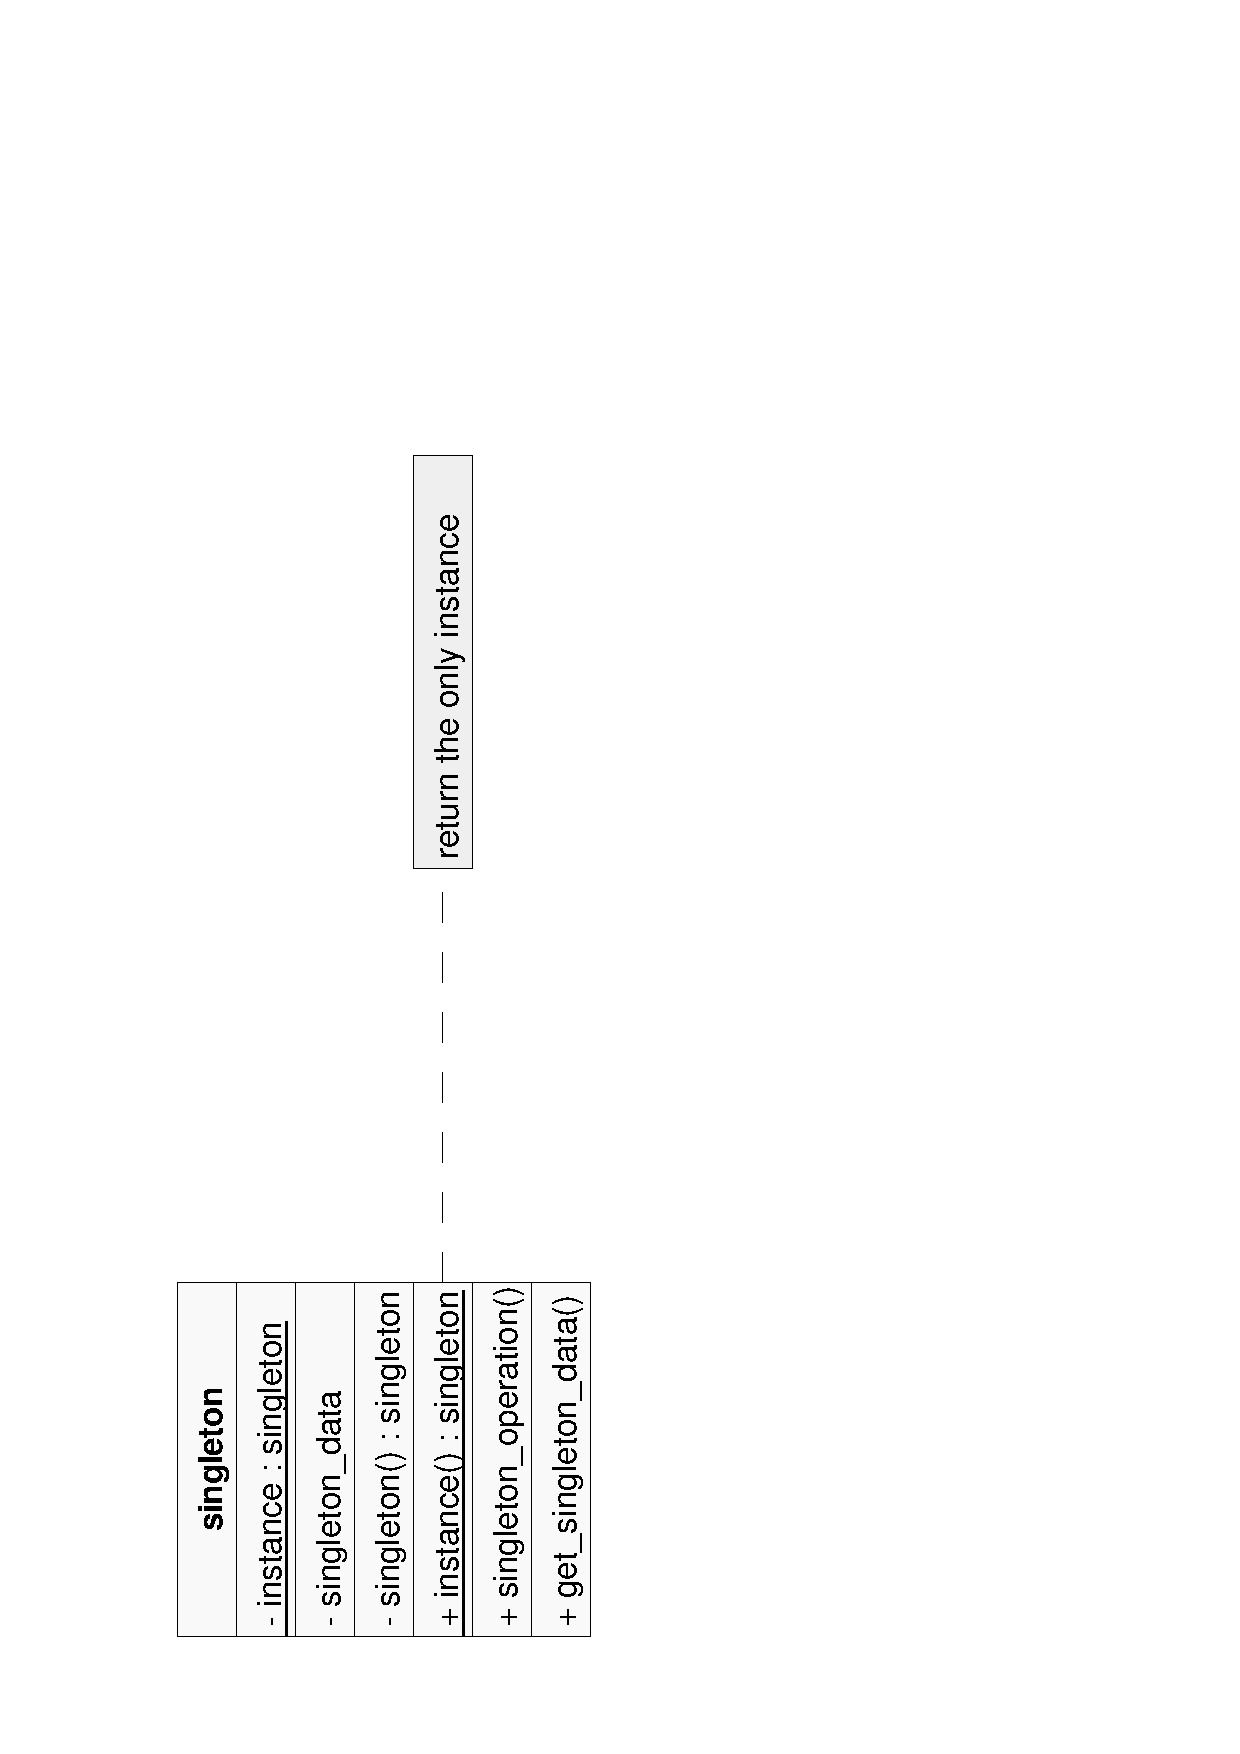
\includegraphics[scale=0.3,angle=-90]{graphic/singleton.pdf}
        \caption{Singleton Pattern}
        \label{singleton_figure}
    \end{center}
\end{figure}

A \emph{Registry} object as described by Fowler \cite{fowler2002} often uses
the \emph{Singleton} pattern, to be unique and to become globally accessible.
Similarly do many so-called \emph{Manager} objects, for example change managers
which are also responsible for the caching of objects.

Global, that is static access -- the main purpose of the \emph{Singleton}
pattern, is its main weakness, at the same time. One obvious solution to avoid
singleton objects could be to forward global information as instances from
component to component, possibly using an own \emph{Lifecycle Method} (section
\ref{component_lifecycle_heading}). This approach, however, might bring with a
rather large number of parameters to be handed over. It therefore seems easier
to use another alternative -- the central tree of knowledge instances, as done
in the interpreter of chapter \ref{cybernetics_oriented_interpreter_heading}.

